\documentclass[8pt]{beamer}
\usepackage[utf8]{inputenc}
\usepackage{listings}
\setbeamertemplate{itemize items}[circle]
\usepackage{scrextend, graphicx, ragged2e}
\usepackage[font=scriptsize]{caption} 

\usetheme{default}
\usecolortheme{rose}

%------------------------------------------------------------
%This block of code defines the information to appear in the
%Title page
\title[Machine-Learining-2\_Project-Presentation\_AS-SS] %optional
{Project Presentation}

\subtitle{Machine Learning 2}

\author[Artur Skowroński, Szymon Socha] % (optional)
{Artur Skowroński, Szymon Socha}

\date[date] % (optional)
\today
%{January 17, 2023}

\logo{
\includegraphics[height=.75cm]{wne-logo-new-en.png}}

%End of title page configuration block
%------------------------------------------------------------



%------------------------------------------------------------
%The next block of commands puts the table of contents at the 
%beginning of each section and highlights the current section:

\begin{document}

\frame{\titlepage}


%---------------------------------------------------------
\begin{frame}
\frametitle{Table of Contents}
\tableofcontents
\end{frame}
%---------------------------------------------------------


\section{Classification}

\subsection{Data}
%---------------------------------------------------------
\begin{frame}
\frametitle{Dataset Description}
The dataset contains 50,000 photos of 43 different German road signs.

Dataset is available on Kaggle (\href{https://www.kaggle.com/datasets/meowmeowmeowmeowmeow/gtsrb-german-traffic-sign}{\underline{here}}).
\begin{figure}[t]
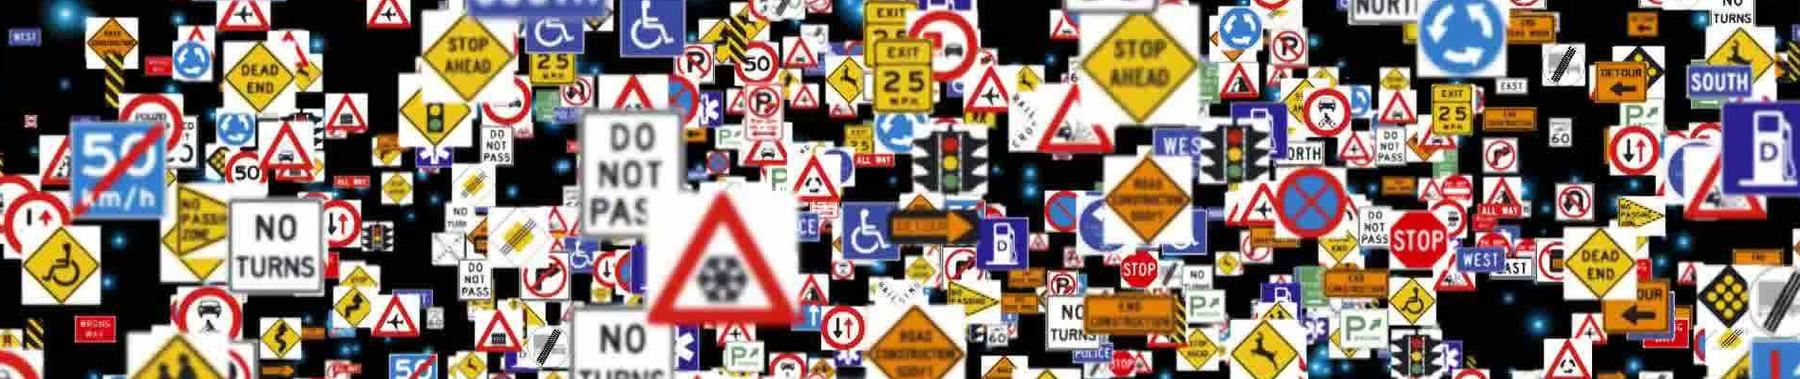
\includegraphics[width=6.5cm, height=3cm]{road-signs.jpg}
\centering
\end{figure}

\end{frame}
%---------------------------------------------------------

\subsection{Data preparation}
%---------------------------------------------------------
\begin{frame}
\frametitle{Data preparation}
At the beginning, we conducted an initial data exploration, which allowed us to conclude that we have an unbalanced dataset. In addition, we have presented sample photos available in the dataset to show that not all signs seem to be very obvious.
As part of the image preprocessing, we took the following steps:
\begin{itemize}
    \item<1-> photos were scaled to a resolution of 32x32
    \item<1-> converted to grayscale
    \item<1-> pixels were flattend and normalized to values between 0-1 
\end{itemize}
Due to the lack of a validation set, it was decided to divide the training set in the proportion of 80\%/20\%. Thanks to this, we have obtained 3 independent harvests.
Then, depending on the algorithm used, we additionally transformed the dependent variable.
\end{frame}
%---------------------------------------------------------

\subsection{Modelling}
%---------------------------------------------------------
\begin{frame}
\frametitle{Modelling part}
We used 3 different classification algorithms for modelling:
\begin{itemize}
    \item<1-> Random Forest
    \item<1-> LightGBM
    \item<1-> CNN (based on LeNet-5 architecture)
\end{itemize}

Accuracy was used as a performance metric, but a confusion matrix and a classification report were also built for each model.\\
\vspace{2mm}
In the case of the first two algorithms, Randomized Search Cross Validation was used to find the optimal hyperparameters.\\
\vspace{2mm}
For neural network, it was decided to use different convolution values and monitored the value of the loss function of the validation set.
\end{frame}
%---------------------------------------------------------

\subsection{Results}
%---------------------------------------------------------
\begin{frame}
\frametitle{Results}
Both the selection of hyperparameters and the training itself took a long time, therefore, when checking, we recommend using the models already saved by us with the appropriate parameters.\\
\vspace{2mm}
\begin{itemize}
    \item<1-> Random Forest\\
    Validation: 61\%; Test: 51\%\\
    \item<1-> LightGBM\\
    Validation: 86\%; Test: 68\%
    \item<1-> CNN (based on LeNet-5 architecture)\\
    Validation: 97\%; Test: 89\%
\end{itemize}
\vspace{2mm}
Possibilities to improve the model:
\begin{itemize}
    \item<1-> Data augmentation
    \item<1-> Creating a larger CNN architecture
    \item<1-> Use of transfer learning*
\end{itemize}

\end{frame}
%---------------------------------------------------------

\section{Regression}

\subsection{Data}
%---------------------------------------------------------
\begin{frame}
\frametitle{Dataset Description}
The dataset contains information about the specifications of laptops and their prices given in Euros. The dataset contains 1320 observations and 13 columns describing the specifications of the laptops:
\begin{itemize}
    \item<1-> \textbf{Company} - \textit{string} - Laptop Manufacturer
    \item<1-> \textbf{Product} - \textit{string} - Brand and Model
    \item<1-> \textbf{TypeName} - \textit{string} -Type (Notebook, Ultrabook, Gaming, etc.)
    \item<1-> \textbf{Inches} - \textit{numeric}- Screen Size
    \item<1-> \textbf{ScreenResolution} - \textit{string} - Screen Resolution
    \item<1-> \textbf{Cpu} - \textit{string} - Central Processing Unit (CPU)
    \item<1-> \textbf{Ram} - \textit{string} - Laptop RAM
    \item<1-> \textbf{Memory} - \textit{string} - Hard Disk / SSD Memory
    \item<1-> \textbf{GPU} - \textit{string} - Graphics Processing Units (GPU)
    \item<1-> \textbf{OpSys} - \textit{string} - Operating System
    \item<1-> \textbf{Weight} - \textit{string} - Laptop Weight
    \item<1-> \textbf{Price euros} - \textit{numeric} - Price (Euro)
\end{itemize}
Dataset is available on Kaggle (\href{https://www.kaggle.com/datasets/muhammetvarl/laptop-price}{\underline{here}}).
\end{frame}
%---------------------------------------------------------

%---------------------------------------------------------
\begin{frame}
\frametitle{Data preparation}
In order to prepare the data, we perform \textbf{EDA}. We also perform \textbf{feature engineering}:
\begin{itemize}
    \item<1-> We extract the screen type and resolution from the \texttt{ScreenResolution} column
    \item<1-> From the \texttt{GPU} column, we extract the processor model and processor clocking
    \item<1-> From the \texttt{Memory} column, we extract whether the laptop has two drives or one, what type and what capacity
\end{itemize}
\vspace{2mm}
We note that the variable \texttt{Price euros} is right-skewed. We logarithmize this variable to give it a distribution closer to the normal distribution.\\
\vspace{2mm}
After feature engineering, we divide the dataset into a training set and a test set. We use the test dataset later \textbf{only} for performance comparison of finished models.\\
\vspace{2mm}
On the training set, we remove one \textbf{outlier}. Originally in the dataset there is one laptop with 64GB RAM, which looks like a very powerful, expensive, gaming laptop. We remove this observation.
\end{frame}
%---------------------------------------------------------


\subsection{Random Forest}
%---------------------------------------------------------
\begin{frame}
\frametitle{Random Forest}
We chose Random Forest as the first algorithm. Even when launching the algorithm with default parameters, the results are promising.\\
The result obtained on the validation set without hyperparameter tuning:\\ \textbf{R\textsuperscript{2}: 90.89\%} \\
\vspace{2mm}
We use \textbf{Randomized Search Cross Validation} to hyperparameter tuning. We improve the model's performance to:\\ \textbf{R\textsuperscript{2}: 92.38\%}\\
\vspace{2mm}
Final Random Forest Regressor model:\\ \texttt{`n\_estimators`: 400, `min\_samples\_split`: 2, `min\_samples\_leaf`: 1, `max\_features`: 'sqrt', `max\_depth`: None, `bootstrap`: False}
\end{frame}
%---------------------------------------------------------


\subsection{XGBoost}
%---------------------------------------------------------
\begin{frame}
\frametitle{XGBoost}
The next algorithm we use is Extreme Gradient Boosting. The result we get on the validation set is very similar to that obtained by Random Forest (slightly worse).\\
The result obtained on the validation set without hyperparameter tuning:\\ \textbf{R\textsuperscript{2}: 90.84\%} \\
\vspace{2mm}
We use \textbf{Randomized Search Cross Validation} to hyperparameter tuning. Thus, we improve the model and obtain a performance better than Random Forest. Obtained score:\\ \textbf{R\textsuperscript{2}: 92.58\%}\\
\vspace{2mm}
Final XGBoost model:\\ \texttt{`colsample\_bytree` = 0.6993051668482431, `eta` = 0.10918301235569373, `gamma` = 0.059657083660437094, `lambdaX` = 0.7857921958527714, `max\_depth` = 9, `min\_child\_weight` = 22.189028104694653, `subsample` = 0.4923455000631808}
\end{frame}
%---------------------------------------------------------


\subsection{Neural Networks}
%---------------------------------------------------------
\begin{frame}
\frametitle{Neural Networks}
The last model we use is Neural Networks. We build a pipeline with \texttt{StandardScaler()} together with Random Search Cross Validation. In order to avoid \textbf{data leakage} we perform scaling on each fold. It is worth mentioning that training the Neural Networks among the three models took the most time - \textbf{more than 3 hours}.\\
The result obtained on the validation set without hyperparameter tuning:\\ \textbf{R\textsuperscript{2}: 79.47\%} \\
\vspace{2mm}
After tuning the hyperparameters, we get a very good model (even too good), which suggests that the model is overfitted (later compare how all models perform on the test set). Obtained score:\\ \textbf{R\textsuperscript{2}: 96.6\%}\\
\vspace{2mm}
Final Neural Networks model:\\ \texttt{`nn3`: 300, `nn2`: 400, `nn1`: 1400, `nl3`: 2, `nl2`: 0, `nl1`: 0, `momentum`: 0.9, `lr`: 0.001, `l2`: 0.1, `l1`: 0, `input\_shape`: 17, `dropout`: 0.3, `decay`: 0, `act`: `relu`}
\end{frame}
%---------------------------------------------------------


\subsection{Performance Comparison}
%---------------------------------------------------------
\begin{frame}
\frametitle{Performance Comparison}
Finally, we compare the performance of previously saved models by doing predictions on a test dataset, \textbf{unseen} by either model.\\
\vspace{2mm}
Test data results:\\
Random Forest R\textsuperscript{2}: \textbf{93.3\%}\\
XGBoost R\textsuperscript{2}: \textbf{91.6\%}\\
Neural Network R\textsuperscript{2}: \textbf{86.5\%}\\
\vspace{2mm}
The model for which we get the best results is \textbf{Random Forest}.\\
\vspace{2mm}
Below is a table with a comparison of model performance with actual values for random observations.
\begin{figure}[t]
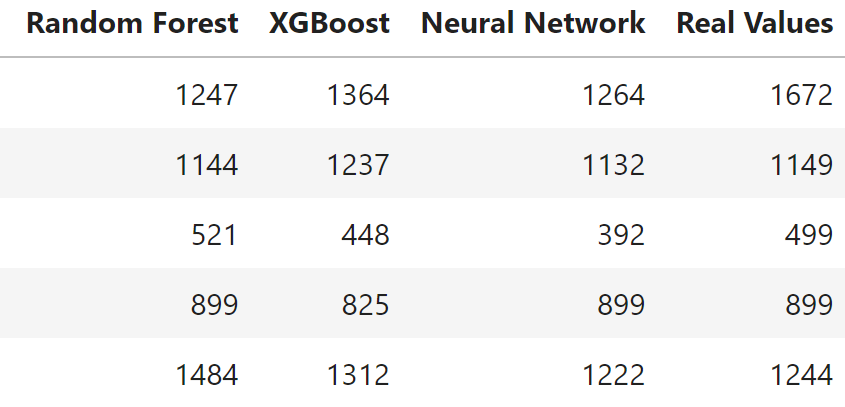
\includegraphics[width=6.5cm]{regression_final_performance_table.png}
\centering
\end{figure}
\end{frame}
%---------------------------------------------------------


\section{Summary}

%---------------------------------------------------------
\begin{frame}
\frametitle{Summary}

\end{frame}
%---------------------------------------------------------


\end{document}
